\documentclass{article}


\usepackage{circuitikz} %Für die Schaltpläne
\usepackage[T1]{fontenc}
\usepackage[utf8]{inputenc}

\usepackage{amsmath}
\usepackage{fancyhdr}
\usepackage{lettrine}
\usepackage{hyperref}
\usepackage{subcaption}
\usepackage{tikz}
\usepackage{cite}
\usepackage{listings}
\usepackage[nottoc, numbib]{tocbibind}
\usepackage{../assets/scripts/tex/color-env}
\usepackage[ngerman]{babel}
%\usepackage{amsmath,amsfonts,stmaryrd,amssymb} % Math packages

\usepackage{enumerate} % Custom item numbers for enumerations

\usepackage[ruled]{algorithm2e} % Algorithms

\usepackage[]{mdframed} % Allows defining custom boxed/framed environments


\mdfdefinestyle{info}{%
	topline=false, bottomline=false,
	leftline=false, rightline=false,
	nobreak,
	singleextra={%
		\fill[black](P-|O)circle[radius=0.4em];
		\node at(P-|O){\color{white}\scriptsize\bf i};
		\draw[very thick](P-|O)++(0,-0.8em)--(O);%--(O-|P);
	}
}

% Define a custom environment for information
\newenvironment{info}[1][Info:]{ % Set the default title to "Info:"
	\medskip
	\begin{mdframed}[style=info]
		\noindent{\textbf{#1}}
}{
	\end{mdframed}
}


\mdfdefinestyle{warning}{
	topline=false, bottomline=false,
	leftline=false, rightline=false,
	nobreak,
	singleextra={%
		\draw(P-|O)++(-0.5em,0)node(tmp1){};
		\draw(P-|O)++(0.5em,0)node(tmp2){};
		\fill[black,rotate around={45:(P-|O)}](tmp1)rectangle(tmp2);
		\node at(P-|O){\color{white}\scriptsize\bf !};
		\draw[very thick](P-|O)++(0,-1em)--(O);%--(O-|P);
	}
}

% Define a custom environment for warning text
\newenvironment{warn}[1][Warning:]{ % Set the default warning to "Warning:"
	\medskip
	\begin{mdframed}[style=warning]
		\noindent{\textbf{#1}}
}{
	\end{mdframed}
}


\usetikzlibrary{shapes}
    \usetikzlibrary{arrows}
    \usetikzlibrary{arrows.meta,topaths}
    \usetikzlibrary{bending}
    \usetikzlibrary{calc}
\title{Elektrotechnik 1 Praktikum 1}


\usepackage[
  includehead,
  headheight = 17mm,
  footskip = \dimexpr\headsep+\ht\strutbox\relax,
  tmargin = 0mm,
  bmargin = \dimexpr17mm+2\ht\strutbox\relax,
]{geometry}

\usepackage{anyfontsize}

\usepackage{xcolor}

\definecolor{DarkGreenBlue}{HTML}{264653}
\definecolor{LightGreenBlue}{HTML}{2A9D8F}
\definecolor{LightOrange}{HTML}{E9C46A}
\definecolor{DarkOrange}{HTML}{F4A261}
\definecolor{RedOrange}{HTML}{E76F51}
\definecolor{BrightRed}{HTML}{D62828}
\definecolor{DeepBlue}{HTML}{003049}

\definecolor{codegreen}{rgb}{0,0.6,0}
\definecolor{codegray}{rgb}{0.5,0.5,0.5}
\definecolor{codepurple}{rgb}{0.58,0,0.82}
\definecolor{backcolour}{rgb}{0.95,0.95,0.92}

\lstdefinestyle{code}{
    backgroundcolor=\color{backcolour},
    commentstyle=\color{codegreen},
    keywordstyle=\color{magenta},
    numberstyle=\tiny\color{codegray},
    stringstyle=\color{codepurple},
    basicstyle=\ttfamily\footnotesize,
    breakatwhitespace=false,
    breaklines=true,
    captionpos=b,
    keepspaces=true,
    numbers=left,
    numbersep=5pt,
    showspaces=false,
    showstringspaces=false,
    showtabs=false,
    tabsize=2
}

\lstset{style=code}


\pagestyle{fancy}
\fancyhead[L]{\leftmark}
\fancyhead[R]{}
\fancyfoot[L]{}
\fancyfoot[C]{\thepage}
\fancyfoot[R]{
\includegraphics[scale=0.2]{../assets/images/haw.jpg}}
\renewcommand\headrulewidth{0.5pt}


\begin{document}


\thispagestyle{empty}
\begin{tikzpicture}[overlay,remember picture]
  \thispagestyle{empty}
  \fill[black!2] (current page.south west) rectangle (current page.north east);

  \begin{scope}[transform canvas ={rotate around ={45:($(current page.north west)+(-.5,-6)$)}}]

    \shade[rounded corners=18pt, left color=DarkGreenBlue, right color=LightGreenBlue] ($(current page.north west)+(-.5,-6)$) rectangle ++(9,1.5);

  \end{scope}

  \begin{scope}[transform canvas ={rotate around ={45:($(current page.north west)+(.5,-10)$)}}]

    \shade[rounded corners=18pt, left color=LightOrange,right color=DarkOrange] ($(current page.north west)+(0.5,-10)$) rectangle ++(15,1.5);

  \end{scope}

  \begin{scope}[transform canvas ={rotate around ={45:($(current page.north west)+(0.5,-10)$)}}]

    \shade[rounded corners=8pt, right color=DarkOrange, left color=LightOrange] ($(current page.north west)+(1.5,-9.55)$) rectangle ++(7,.6);

  \end{scope}

  \begin{scope}[transform canvas ={rotate around ={45:($(current page.north)+(-1.5,-3)$)}}]

    \shade[rounded corners=12pt, left color=DeepBlue!80, right color=DeepBlue!60] ($(current page.north)+(-1.5,-3)$) rectangle ++(9,0.8);

  \end{scope}

  \begin{scope}[transform canvas ={rotate around ={45:($(current page.north)+(-3,-8)$)}}]

    \shade[rounded corners=28pt, left color=BrightRed, right color=BrightRed!80] ($(current page.north)+(-3,-8)$) rectangle ++(15,1.8);

  \end{scope}

  \begin{scope}[transform canvas ={rotate around ={45:($(current page.north west)+(4,-15.5)$)}}]

    \shade[rounded corners=25pt, left color=RedOrange, right color=DarkOrange] ($(current page.north west)+(4,-15.5)$) rectangle ++(30,1.8);

  \end{scope}

  \begin{scope}[transform canvas ={rotate around ={45:($(current page.north west)+(13,-10)$)}},]

    \shade[rounded corners=22pt, left color=DeepBlue,right color=DarkGreenBlue] ($(current page.north west)+(13,-10)$) rectangle ++(15,1.5);

  \end{scope}

  \begin{scope}[transform canvas ={rotate around ={45:($(current page.north west)+(18,-8)$)}},]

    \shade[rounded corners=8pt, left color=DarkOrange] ($(current page.north west)+(18,-8)$) rectangle ++(15,0.6);

  \end{scope}

  \begin{scope}[transform canvas ={rotate around ={45:($(current page.north west)+(19,-5.65)$)}},]

    \shade[rounded corners=12pt, left color=RedOrange] ($(current page.north west)+(19,-5.65)$) rectangle ++(15,0.8);

  \end{scope}

  \begin{scope}[transform canvas ={rotate around ={45:($(current page.north west)+(20,-9)$)}}]

    \shade[rounded corners=20pt, left color=BrightRed, right color=BrightRed!80] ($(current page.north west)+(20,-9)$) rectangle ++(14,1.2);

  \end{scope}

  \draw[ultra thick,gray] ($(current page.center)+(5,2)$) -- ++(0,-3cm) node[midway,left=0.25cm,text width=5cm,align=right,black!75]{{\fontsize{25}{30} \selectfont \bf GEP\\[10pt] Praktikum 2}} node[midway,right=0.25cm,text width=6cm,align=left,orange]{{\fontsize{70}{86} \selectfont 2021}};

  \node at ($(current page.center)+(0,-4)$) {{\fontsize{40}{72} \selectfont B6-Brücke}};

  \node[text width=8cm,align=center] at ($(current page.center)+(0,-6.5)$) {{\fontsize{16}{20} \selectfont \textcolor{orange}{ \bf 7. Dezember 2021}} \\[3pt] Emily Antosch 2519935};

\end{tikzpicture}

\newpage


\tableofcontents

\listoffigures

\lstlistoflistings

\newpage

\section{Einführung}

In diesem Versuch wollen wir uns mit der netzgeführten B6-Brücke beschäftigen. Dabei wollen wir sowohl eine ohmsche als auch eine ohmsch-induktive Last untersuchen und unsere Ergebnisse mit verschiedenen Messgeräten festhalten. 

\newpage

\section{Vorbereitung}

Wir wollen uns zunächst über den Aufbau der B6-Brücke klar werden:
\begin{figure}[h]
  \centering
  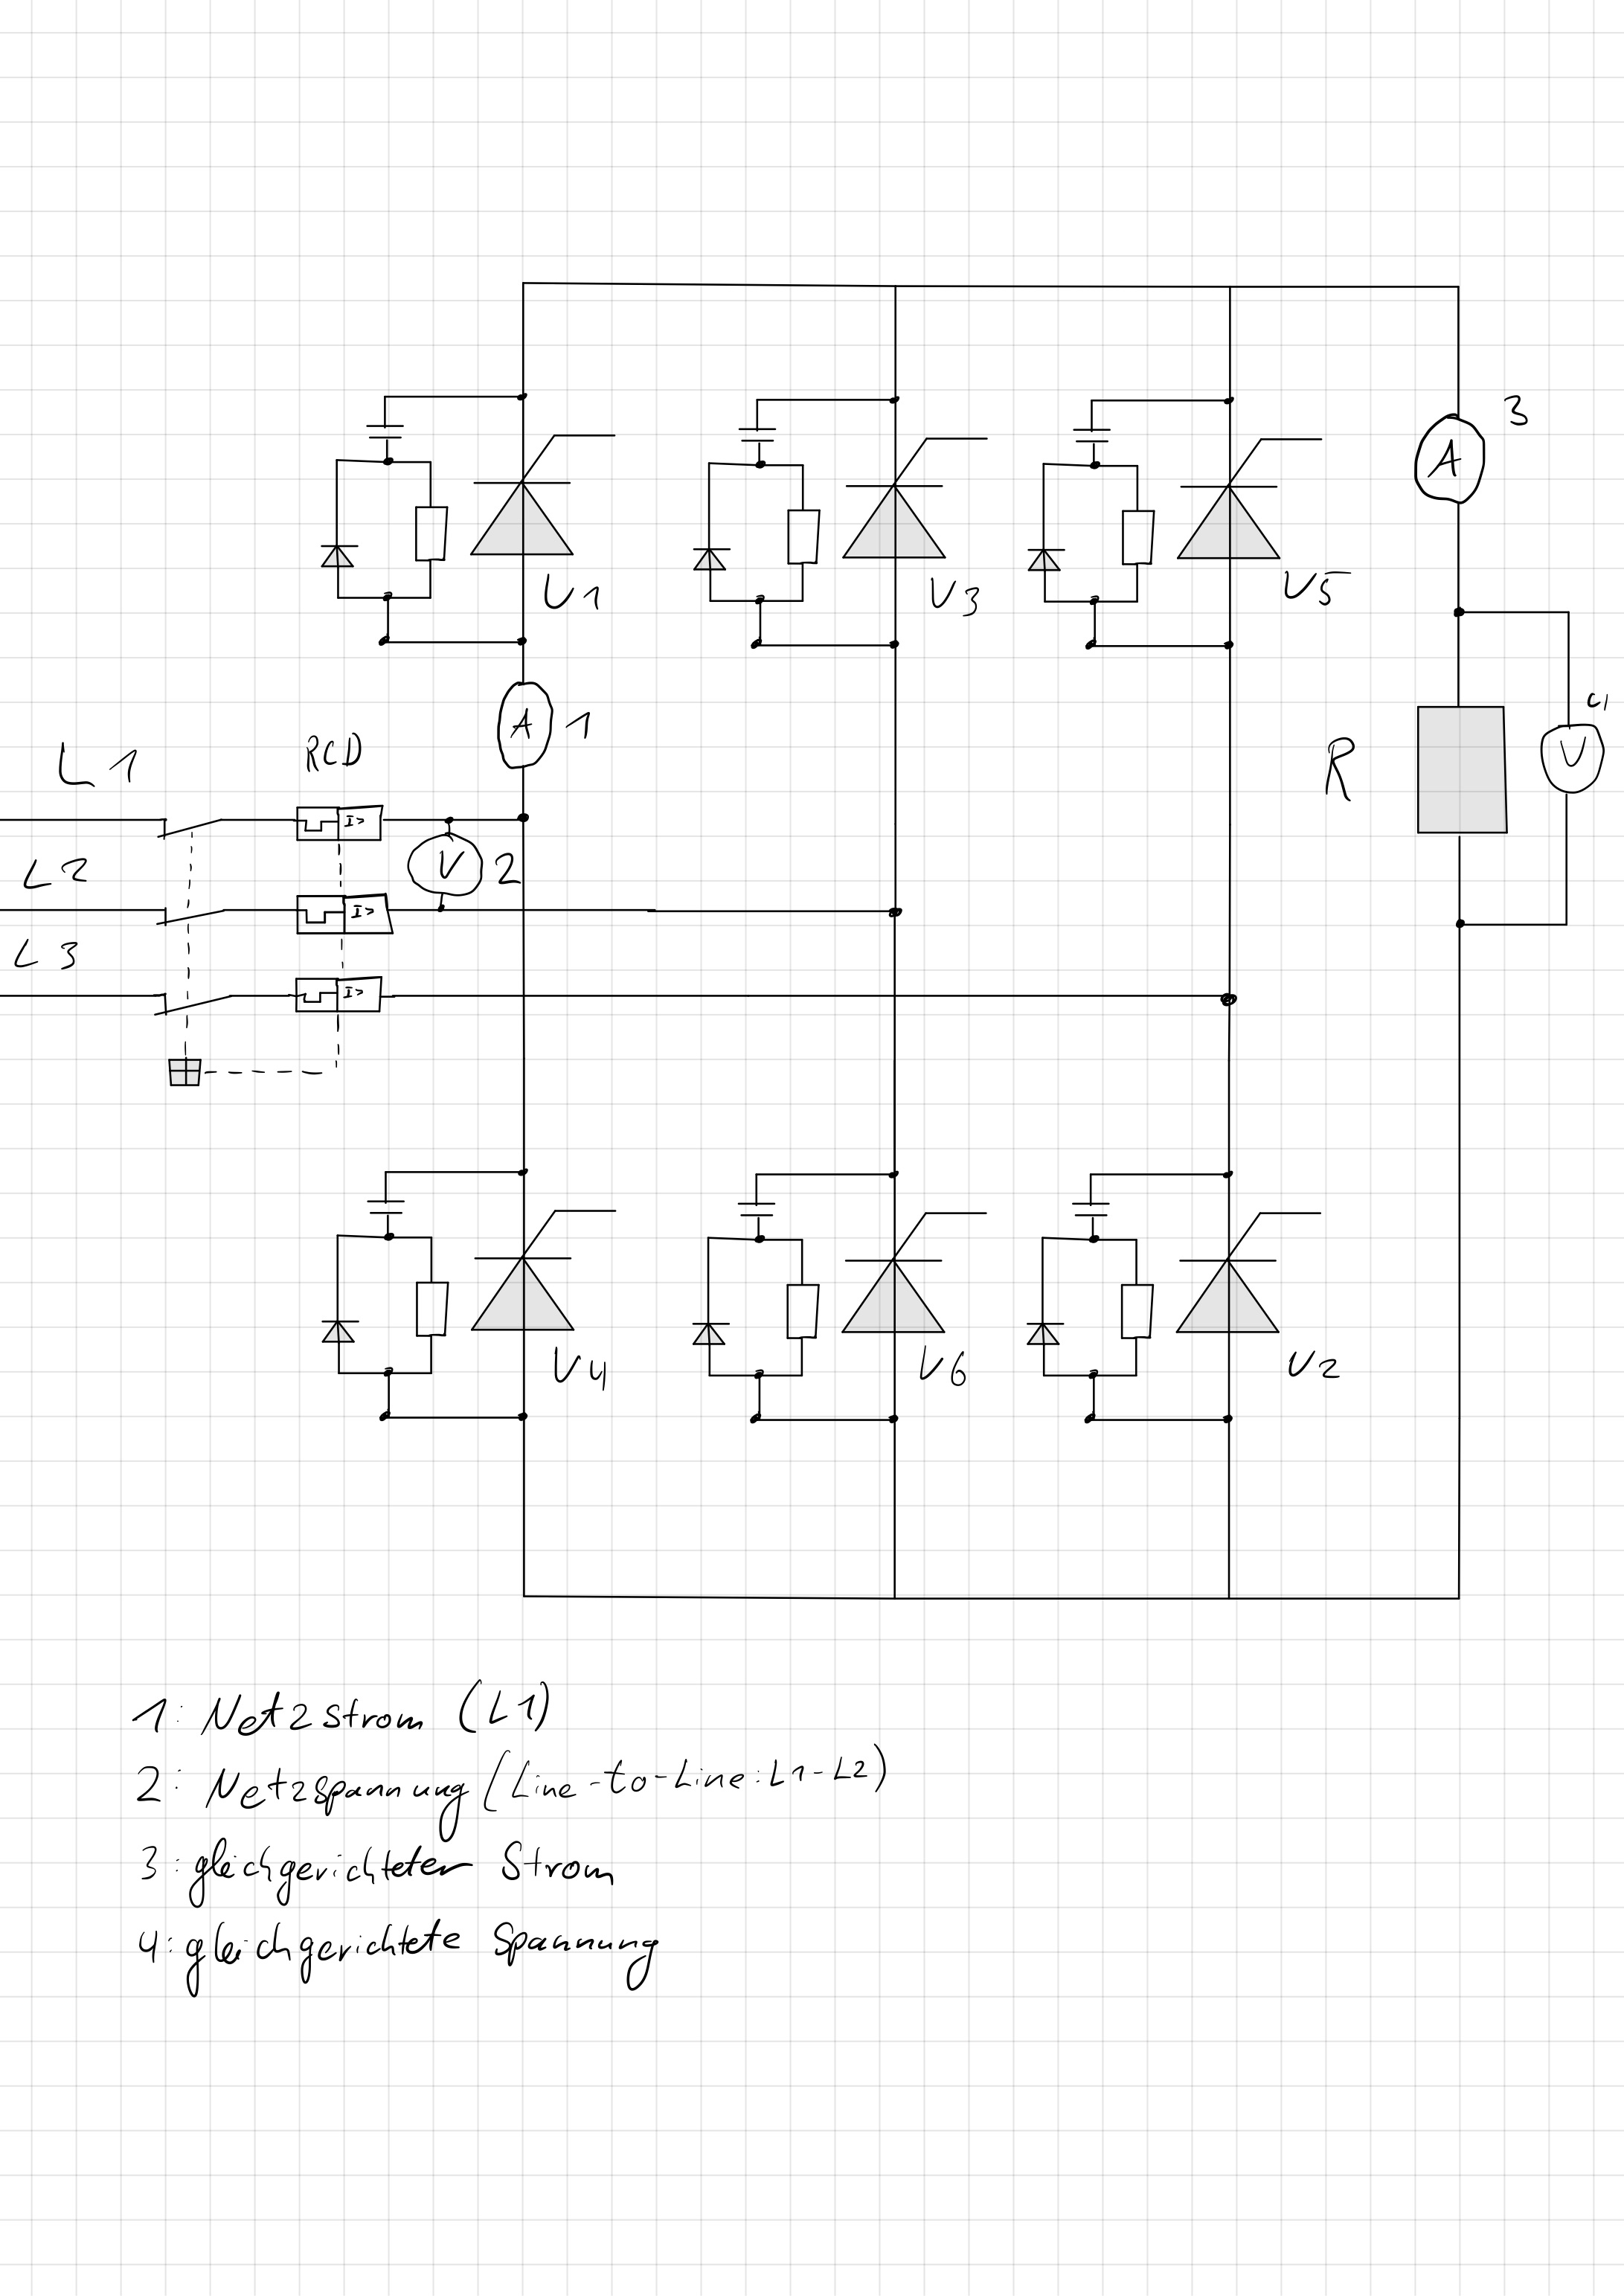
\includegraphics[width=0.8\textwidth]{../assets/images/GEP2/b6.jpg}
  \caption{Aufbau der B6-Brücke}
  \label{fig:b6}
\end{figure}

Zusätzlich wollen wir uns im Vorfeld überlegen, inwieweit wir sicherstellen können, dass die vorgegebenen Werte eingehalten werden können. Mit $U_{S} = 26V$ und $I_{d,max} = 2A$ können wir nun bei maximaler Aussteuerung der Schaltung, also bei $\alpha = 0^{^{\circ}}$, die maximale Spannung $$U_{i\alpha} = \frac{3\cdot \sqrt{2}}{\pi}\cdot U_{L} \cdot cos(0^{\circ}) = \frac{3\cdot \sqrt{2}}{\pi}\cdot 26V = 60.816V$$
berechnen. Um nun eine ohmsche Last zu berechnen, die die Schaltung in diesen Werten beschränkt rechnen wir

\begin{equation*}
  \label{eq:1}
  R_{L} = \frac{U_{i\alpha}}{I_{d,max}} = \frac{60,816V}{2A} = 30.4 \Omega
\end{equation*}

\section{Messreihe}

\subsection{Messung der Steuerspannung und der gleichgerichteten Spannung}

Wir wollen zunächst unseren Offset bei der Einstellung unseres Zündverzögerungswinkels ermitteln. Dabei stellen wir unsere Steuerspannung $U_{St} = 10V$ auf das Maximum ein und messen vom Nulldurchgang der Spannung $U_{21}$ zur ersten Zündung. Wir erhalten eine Verzögerung von $\Delta t = 3.68ms$, damit rechnen wir

\begin{equation*}
  \label{eq:2}
  \Delta\alpha = \Delta t \cdot 360^{\circ} \cdot \frac{1}{T} - 60^{\circ} = 3.68ms \cdot 360^{\circ} \cdot \frac{1}{20ms} - 60^{\circ} = 6,2^{\circ}
\end{equation*}

und erhalten damit den Winkel, den wir bei der minimalen Einstellung unseres Zündwinkeltransformators haben. Alle weiteren Messungen basieren dann auf diesem Offset. Der Bild auf dem Oszilloskop ist dann unten noch einmal dargestellt:

\begin{figure}[h]
  \centering
  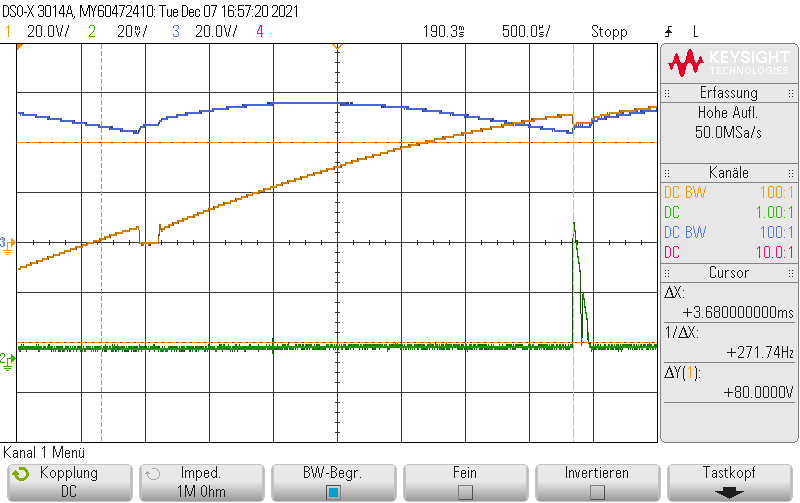
\includegraphics[width=\textwidth]{../assets/images/GEP2/startAngle.png}
  \caption{Startmessung des Winkels bei 10V}
  \label{fig:startAngle}
\end{figure}

Wir wollen nun uns die Tabelle der Werte einmal anschauen:

\begin{table}[h]
  \centering
  \begin{tabular}{|c|c|c|}
    $\alpha$ & $U_{St}$ & $U_{i\alpha}$ \\
    $6,2^{\circ}$ & & \\
  \end{tabular}
  \caption{Messreihe der Steuerspannung und der gleichgerichteten Spannung im Bezug auf den Zündverzögerungswinkel}
  \label{tab:mess1}
\end{table}

\end{document}
